\section{LEP and the OPAL detector}
\subsection{LEP}
%LEP luftaufnahme
\begin{figure}[ht]
	\centering
	\includegraphics[width=1.0\linewidth]{graphics/LEPmap}
	\caption[Bird's eye view LEP]{Bird's eye view of the Large Electron-Positron Collider at Cern in Geneva, Switzerland. Today, the large circular collider tunnel is used for the Large Hadron Collider (LHC)\cite{jakobs}. The smaller circle belonged to the Super Proton Synchroton (SPS) experiment.}
	\label{fig:LEPmap}
\end{figure}
The Large Electron-Positron Collider is storage ring with a diameter of 27 km. It accelerated 4 bunches of $4\cdot 10^{11}$ electrons and positrons in opposite directions for about 20 hours. At four predetermined points (the positions of the detectors: Aleph, Delphi, L3 and OPAL) the beams collided about every 25$\mu s$, but the reaction $e^+ e^- \rightarrow f \bar{f}$ only occurred at a frequency of roughly 1Hz \cite{muenchen}.

\subsection{OPAL}
The OPAL detector consists of several components arranged in a shell-like manner(s.figure \ref{fig:OPALaufbau}). Closest to the beam is the central tracking chamber (red), enabling tracking of charged particles. It is followed by the electromagnetic calorimeter (cyan), which is used to determine the energy of positrons, electrons and photons.
Next is the hadronic calorimeter (yellow), measuring the energy of hadrons passing through the electromagnetic calorimeter.
The outermost shell are the muon detectors(blue), which, as the name suggests, are used to detect muons \cite{cern}.\\

%schematischer OPAL-Aufbau
\begin{figure}[ht]
\centering
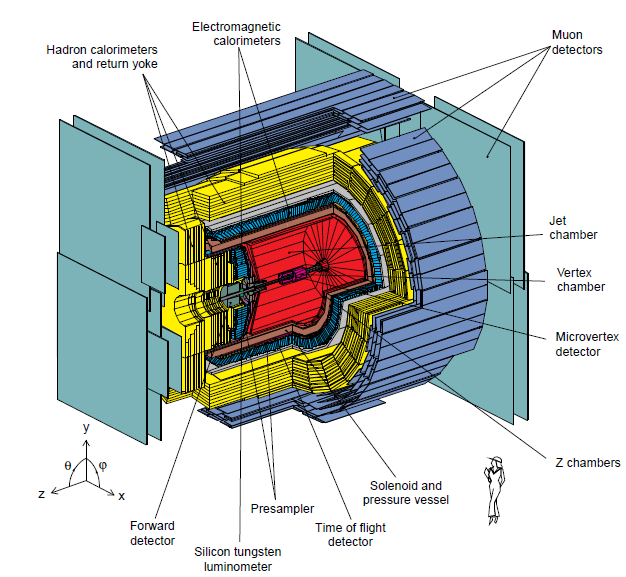
\includegraphics[width=1.0\linewidth]{graphics/OPALaufbau}
\caption[Opal schematic build up]{Schematic structure of the opal detector. The different types of detecting units are arranged in shells around the beam path. \cite{cern}}
\label{fig:OPALaufbau}
\end{figure}

\paragraph{Tracking chamber:}
A charged particle passing through the detector ionizes atoms of the filling gas. The freed electrons (primary electrons) are accelerated towards anode wires spanned between two cathode plates and ionize more atoms, thus creating a shower of secondary electrons.
Each of the anode wires can be read out separately. At constant drift velocities, the time difference between the passing of the (charged) particle and the response of the wire is proportional to the distance of the track. One can determine the track by measuring those time differences.
The chamber is additionally surrounded by a coil creating a magnetic field parallel to the $e^+e^-$-beam, thus forcing the charged particles on a circular trajectory. From the radius of this trajectory one can infer the particle's momentum \cite{staatsex}.
%elektromagnetisches Kaloriemeter

\paragraph{Electromagnetic Calorimeter:}
OPAL's electromagnetic calorimeter is a total absorption calorimeter mostly made of lead-glass blocks \cite{cern}. High energy electrons and photons passing through the detector lose energy primarily due to bremsstrahlung (electron) and pair production (photon). The created secondary particles also lose energy this way, resulting in showers of particles, each generation with less energy. The shower ends when the energy of those particles is lower than the critical energy $E_C$ at which the energy of electrons due to bremsstrahlung is equal to the loss due to ionization. The deposited energy is proportional to the energy of the original particle \cite{muenchen}.

\paragraph{Hadronic Calorimeter:}
The principle is the same as above, but instead of bremsstrahlung and pair production, a different effect causes the showers.. A hadronic shower forms when a strongly interacting particle hits an absorber: in a series of inelastic collisions with the nuclei of the absorber, secondary hadrons are created, which also are scattered inelastically. The cascade stops once the particles have so little energy that they can be absorbed completely.
\paragraph{Muon detector:}
The Muon detector consists of 4 layers of muon chambers. They function like the tracking chamber but since all other charged particles are absorbed in the previous shells, only muons leave a track in this detector \cite{muenchen}.